\documentclass{beamer}
\usepackage{amsmath,amssymb,amsthm,slashed, euscript}
\usepackage{mathrsfs} 

\usepackage{tikz}
\usepackage{tikz-cd}

%\usepackage{mathtools}

\usetikzlibrary{matrix}
\usetikzlibrary{cd}


\textwidth=110mm


\title{Hausdorff blowing-up of spectra of $C^*$-algebras and its applications}
\institute
{
Algebras in analysis
}

\author{Petr R. Ivankov  }



\theoremstyle{plain}
\newtheorem{defn}{Definition}
\newtheorem{rem}{Remark}
\newtheorem{exm}{Example}
\newtheorem*{claim}{Claim}
\newtheorem{prop}{Proposition}
\newtheorem{empt}[prop]{}%[section]
\newtheorem{lem}{Lemma}%[section]
\newtheorem{thm}{Theorem}%[section]



\newcommand{\A}{\mathcal{A}}
\newcommand{\be}{\begin{equation}}
\newcommand{\ee}{\end{equation}}
\newcommand{\Ga}{\Gamma}
\newcommand{\B}{\mathcal{B}}
\newcommand{\Cc}{\mathcal{C}}
\newcommand{\C}{\mathbb{C}}
\newcommand{\D}{\mathcal{D}}
\newcommand{\G}{\mathcal{G}}
\newcommand{\Hc}{\mathcal{H}}
\newcommand{\Lc}{\mathcal{L}}
\newcommand{\Pc}{\mathcal{P}}
\newcommand{\Sc}{\mathcal{S}}
\newcommand{\U}{\mathcal{U}}
\newcommand{\rar}{\rightarrow}
\newcommand{\Ef}{\mathbb{E}}
\newcommand{\desc}{\mathfrak{desc}}

\newcommand{\ga}{\gamma} 
%Uppercase Gothic characters
\newcommand{\gtA}{\mathfrak{A}}
\newcommand{\gtB}{\mathfrak{B}}
\newcommand{\gtM}{\mathfrak{M}}
\newcommand{\gtN}{\mathfrak{N}}
\newcommand{\gtP}{\mathfrak{P}}
\newcommand{\gtS}{\mathfrak{S}}

%Lowercase Gothic characters
\newcommand{\gtf}{\mathfrak{f}}
\newcommand{\gtg}{\mathfrak{g}}
	\newcommand{\End}{\mathrm{End}}       %%

%Bold Characters
\newcommand{\Cb}{\mathbb{C}}
\newcommand{\Nb}{\mathbb{N}}
\newcommand{\Rb}{\mathbb{R}}
\newcommand{\Zb}{\mathbb{Z}}

%Uppercase Greek characters
\newcommand{\Gm}{\Gamma}
\newcommand{\Te}{\Theta}
\newcommand{\Om}{\Omega}
\newcommand{\s}{ }

%Lowercase Greek characters
\newcommand{\al}{\alpha}
\newcommand{\gm}{\gamma}
\newcommand{\dl}{\delta}
\newcommand{\sg}{\sigma}
\newcommand{\ph}{\varphi}
\newcommand{\te}{\theta}
\newcommand{\ze}{\zeta}
\newcommand{\lift}{\mathfrak{lift}}
\newcommand{\eps}{\varepsilon}                    %% tensor product


\newcommand{\Id}{\mathrm{Id}}
\newcommand{\Aut}{\mathrm{Aut}}
\newcommand{\Coo}{{\mathrm{C}}^\infty}
\newcommand{\alg}{\mathrm{alg}}
\newcommand{\diag}{\mathrm{diag}}
\newcommand{\spinc}{\textbf{$spin^c$}}
\newcommand{\Hom}{\mathrm{Hom}}
\newcommand{\supp}{\mathrm{supp}}
\newcommand{\Ccl}{\mathbf{C}l}
\newcommand{\xto}{\xrightarrow}
\newcommand{\T}{\mathbb{T}} 
\newcommand{\lto}{\longrightarrow}
\newcommand{\ox}{\otimes}
\newcommand{\nb}{\nabla}
\newcommand{\sS}{\mathcal{S}}
\newcommand{\Dn}{D\!\!\!\!/}
%\newcommand{\ij}{{i,j}}
\newcommand{\aC}{\ensuremath{\underline{\Cb}} }
\newcommand{\scp}[2]{\left\langle{#1},{#2}\right\rangle}
\newcommand{\op}[1]{J{#1}J^\dag}
\newcommand{\sA}{\mathcal{A}} 
\newcommand{\sB}{\mathcal{B}}       %%
\newcommand{\sC}{\mathcal{C}}       %%
\newcommand{\sD}{\mathcal{D}}       %%
\newcommand{\sE}{\mathcal{E}}       %%
\newcommand{\sF}{\mathcal{F}}       %%
\newcommand{\sG}{\mathcal{G}}       %%
\newcommand{\sH}{\mathcal{H}}       %%
\newcommand{\sI}{\mathcal{I}}       %%
\newcommand{\sJ}{\mathcal{J}}       %%
\newcommand{\sK}{\mathcal{K}}       %%
\newcommand{\sL}{\mathcal{L}}       %%
\newcommand{\sM}{\mathcal{M}}       %%
\newcommand{\sN}{\mathcal{N}}       %%
\newcommand{\sO}{\mathcal{O}}       %%
\newcommand{\sP}{\mathcal{P}}       %%
\newcommand{\sQ}{\mathcal{Q}}       %%
\newcommand{\sR}{\mathcal{R}}       %%
\newcommand{\sT}{\mathcal{T}}       %%
\newcommand{\sU}{\mathcal{U}}       %%
\newcommand{\sV}{\mathcal{V}}       %%
\newcommand{\sX}{\mathcal{X}}       %%
\newcommand{\sY}{\mathcal{Y}}       %%
\newcommand{\sZ}{\mathcal{Z}}       %%
\newcommand{\N}{\mathbb{N}}                  %% 

\renewcommand{\a}{\alpha}     
\newcommand{\la}{\lambda}     
\newcommand{\La}{\Lambda}
\newcommand{\bt}{\beta}           %% short for  \beta
 \renewcommand{\H}{\mathcal{H}}               %% Hilbert space
 
 	\newcommand{\bean}{\begin{eqnarray*}}
 	\newcommand{\eean}{\end{eqnarray*}}
    
\newcommand{\bydef}{\stackrel{\mathrm{def}}{=}}  
\newcommand{\hookto}{\hookrightarrow}        %% abbreviation
  \usepackage{graphicx}
  \graphicspath{ {./images/} }
  \usepackage{tikz}
\usetikzlibrary{calc,trees,positioning,arrows,chains,shapes.geometric,%
	decorations.pathreplacing,decorations.pathmorphing,shapes,%
	matrix,shapes.symbols}
	
	\usetikzlibrary{trees,positioning,shapes,shadows,arrows}
  

\tikzset{
	basic/.style  = {draw, text width=2cm, drop shadow, font=\sffamily,     rectangle},
	root/.style   = {basic, rounded corners=2pt, thin, align=center,
		fill=green!30},
	level 2/.style = {basic, rounded corners=6pt, thin,align=center,     fill=green!60,
		text width=8em},
	level 3/.style = {basic, thin, align=left, fill=pink!60, text width=6.5em}
}
\begin{document}
%\titlepage
\begin{frame}
  \titlepage
\end{frame}
\section{Hausdorff blowing-up}
\begin{frame}
	\begin{definition}\label{blowing_u_defn}\alert{Petr Ivankov.}
		If $A$ is a $C^*$-algebra then \alert{Hausdorff blowing-up} is an inclusion  $C_0\left( \sY\right) \subset M\left( A\right)$ of commutative $C^*$-algebra such that:
		\begin{enumerate}
			\item[(a)] $C_c\left( \sY\right)A$ is dense in $A$,
			\item [(b)]  $AC_c\left( \sY\right)$ is dense in $A$.
		\end{enumerate} 
	\end{definition}
	\begin{rem}
		Both conditions (a) and (b) are equivalent to each other and are used for convenience.
	\end{rem}
	\begin{rem}
		If $C_0\left( \sY\right)$ is within a center of $M\left( A\right)$ then $\sY$ is the spectrum of $A$.
	\end{rem}
	\begin{rem}
		The "\alert{blowing-up}" etymology comes from the algebraic geometry, where it means a map from nonsingular variety  onto a variety with singularities.
	\end{rem}
\end{frame}
\begin{frame}
\huge{Example} \normalsize	 $$C_c\left(M \right) \subset M\left( C^*\left(M, \sF \right)\right) $$  where 
	$\left(M, \sF \right)$ is a foliated manifold and  $C^*\left(M, \sF \right)$ is a $C^*$-algebra of foliation. The spectrum of $C^*\left(M, \sF \right)$ is a set of leaves, and there is the natural map from $M$ to the spectrum.
\\
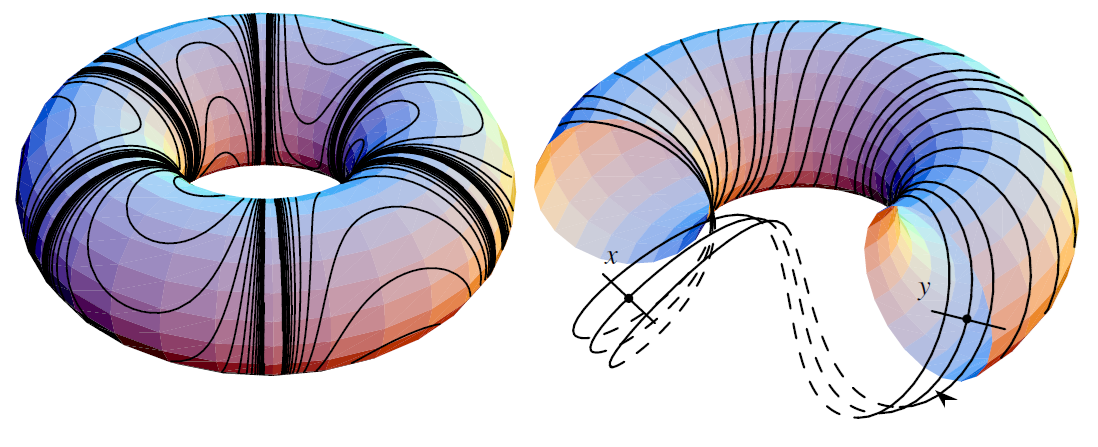
\includegraphics[scale=0.25]{Untitled.png}
\begin{rem}
There are different of versions of $ C^*\left(M, \sF \right)$, all of them are being studied.
\end{rem}
\end{frame}
\begin{frame}
	\huge{Simplest analogy} \normalsize\\
There are several  analogies of Hausdorff blowing-up  with spectrum.\\
Spectrum
$$
C_0\left(\sX_1\sqcup ...\sqcup \sX_n \right) \cong C_0\left(\sX_1 \right) \oplus ...\oplus C_0\left(\sX_n \right) 
$$
Blowing-up
\bean
C_0\left( \sY_1\sqcup ...\sqcup \sY_n\right)\subset M\left( A\right)\quad   
A \cong A_1\oplus ...\oplus A_n,\\
\forall j \in \{1,...,n\}\quad C_0\left(\sY_j \right) \subset M\left(A_j \right). 
\eean

\end{frame}

\begin{frame}
	\begin{thm}\label{pedersen_ideal_thm} \alert{Pedersen G.K.}
		% THEOREM 5.6.1
		For each $C^*$-algebra $A$ there is a dense hereditary ideal $K(A)$,
		which is minimal among dense ideals.
		
	\end{thm}
	\begin{proof}
		Let $K(]0, \infty [)$ denote the set of continuous functions on $]0, \infty [$ with 
		compact support and define 
		\be\label{pedersen_k0_eqn}
		K\left( A \right)_0 \bydef \left\{f\left(x\right) \left|x \in A_+, \quad f \in K(]0, \infty [) \right.\right\}.
		\ee
		Let 
		\be\label{pedersen_k_plus_eqn}
		K\left( A \right)_+ \bydef \left\{x \in A_+ \left|x \le \sum_{j = 1}^nx_j, \quad x_j \in  	K\left( A \right)_0\right.\right\}, 	
		\ee
		so that $	K\left( A \right)_+$ is the smallest hereditary cone  containing $K\left( A \right)_0$. If $K(A)$ 
		is  the algebraic  $\C$-linear span of $K(A)_+$ then $K(A)$,
		which is minimal among dense ideals. The full  proof is  described in Pedersen's book.
	\end{proof}
	
\end{frame}

\begin{frame}
	The above ideal is said to be \alert{Pedersen's ideal}. It is  proven by \alert{Petr Ivankov} that $f \in K(]0, \infty [)$ can be replaced with the continuous functions given by
		$$
		f_\eps\left( x\right)  \bydef\left\{
		\begin{array}{c l}
			0 &x \le \eps \\
			x - \eps & x > \eps
		\end{array}\right.
	$$
	where $\eps > 0$.
\end{frame}


\begin{frame}
\huge{Pedersen's ideal and compact support}\normalsize\\ 
	If $A$ is a $C^*$-algebra with Hausdorff spectrum then for any $a\in A$ there is generated by $a$ closed two sided ideal $I\subset A$. The ideal yields an open subset of the spectrum of $A$ the closure of this set is the \alert{support} $\supp~a$ of $a$. It is well known  that if $a \in K\left(A \right)$ then  $\supp~a$ is compact. There is a generalization of this result.
\end{frame}
\begin{frame}
\begin{definition}\label{blowing_ideals_au_ua_defn}\alert{Petr Ivankov}
	Let  $ C_0\left(\sY\right)\subset  M\left( A\right) $ be  Hausdorff blowing-up of $A$, and let $\sU \subset \sY$ be an open subset. Both left and right  closed ideals $A_\sU$  and $_\sU A$ of $A$ which are   generated by sets 	$AC_0\left( \sU\right)$ and $C_0\left( \sU\right)A$ are the \alert{left} $\sU$-\alert{ideal} and the \alert{right} $\sU$-\alert{ideal} respectively. A hereditary $C^*$-subalgebra of $A$ given by
	\bean
	\begin{split}
		_\sU A_\sU \bydef		_\sU A\cap  A_\sU = A^*	_\sU \cap  A_\sU
	\end{split}
	\eean	
	is the \alert{hereditary} $\sU$-\alert{subalgebra}.
	
	\end{definition}
	
	\begin{definition}\label{blowing_support_defn}
		If $C_0\left( \sY\right) \subset M\left(A \right)$ is    {Hausdorff blowing-up} of $A$,  $a \in A$ and
		$
		\sU_a \bydef\bigcap 
		\left\{\left.{\sU} \subset \sX\right| a\in~_\sU A_{\sU} \right\}
		$
		then the  closure $\sV_a$  of $\sU_a$ is said to be the \alert{support} of $a$. We write $\supp~ a \bydef \sV_a$. This definition is a generalization of the definition of support in case of $C^*$-algebra with Hausdorff spectrum. 
	\end{definition}
	
\end{frame}

\begin{frame}
	\begin{lemma}\label{blowing_pedersen_compact_lem}
		If  $C_0\left( \sY\right)\hookto M\left( A\right)$ is Hausdorff blowing-up and $a\in A$ belongs to the Pedersen's ideal $K\left(A \right)$  then the support $\supp~a$ of $a$  is compact.
	\end{lemma}
\begin{proof}	
If $a \in K\left(A\right)_0$  then  there is $\eps > 0$ and $b \in A_+$ such that $a = f_\eps \left( b\right)$. On the other hand  there is a positive element  $c= f^*bf\in  A_+$  such that  $f\in C_c\left(\sY \right)$, $\left\|f \right\|=1 $, $c < b$, $\left\|c - b \right\|  < \eps/2$, and $\supp~ c\subset \supp ~f$ is compact.
If $a \le c$ does not hold and $\rho: A \hookto B\left(\H \right)$ is a faithful  nondegenerate representation  then there is $\xi \in \H$ such that
\bean
 \left( \xi, \rho\left( a \right) \xi\right) > \left( \xi, \rho\left( c \right) \xi\right)
\eean
From $\left\|c - b \right\|  < \eps/2$ if follows that
\bean
\forall \xi \in \H  \quad \left\| \xi \right\| = 1\quad \Rightarrow\quad  \left|\left( \xi, \rho\left( b \right) \xi\right)-\left( \xi, \rho\left( c \right) \xi\right) \right| < \eps/2
\eean
\end{proof}

\end{frame}
\begin{frame}
On the other hand from $a =f_\eps \left( b\right)> 0$ it follows that there is $\xi \in H$ and $\la \in \mathbf{R}_+$ such that
\bean
\left\| \xi \right\| = 1,\\
\rho\left(a \right) \xi = \la \xi,\\
\rho\left(b \right)\xi = \left( \la+\eps \right) \xi,\\
\rho\left(a \right)\xi = \la  \xi,\\
\left( \xi, \rho\left( b \right) \xi\right) - \left( \xi, \rho\left( a \right) \xi\right)= \\=\eps
\left( \xi, \rho\left( c \right) \xi\right)- \left( \xi, \rho\left( a \right) \xi\right)> \frac{\eps}{2}
\eean

Above condition contradicts with
$$
\forall \xi\in \H \quad\left|\left( \xi, \rho\left( b \right) \xi\right)-\left( \xi, \rho\left( c \right) \xi\right) \right| < \eps/2
$$
so $a \le c$.
If $\supp a \subsetneqq \supp c$ then there is a nonempty  open set  $\sU \subset \supp~ a\setminus \supp~ c$. For any $f \in C_0\left(\sU \right)\setminus \{0\}$ one has
\bean
faf^* > 0,\\
fcf^* = 0.
\eean
\end{frame}
\begin{frame}
However it is impossible since $a \le c$, so $\supp~ a \subsetneqq \supp ~c$ is not true and $\supp ~a \subset\supp ~c$. Thus the set $\supp~ a$ is a closed subset of the compact set $\supp~ c$ therefore $\supp~ a$ is compact. Using this fact and the definition of the Pedersen's ideal we conclude that $\supp~ a$ is compact for any $a \in K\left( A\right)$. 
	
	
\end{frame}
\begin{frame}
\section{Physical issues}
\huge{Physical issues} \normalsize

\begin{enumerate}
	\item 	Experimentally proved low-energy physics is related to $C^*$-algebras with Hausdorff spectrum.
	\item 		Experimentally proved physics is not self-consistent since it contains high-energy  divergent integrals.
	\item Divergent integrals are caused by shooting toward a point. In non-Hausdorff spaces there is no tendency towards a point.
	\item To avoid divergences one needs application of $C^*$-algebras with non-Hausdorff spectrum.
	\item Hausdorff blowing-up yields a duality between $C^*$-algebras with Hausdorff spectrum and non-Hausdorff one.
	\item Hausdorff blowing-up has the following physical meaning. A noncommutative $C^*$-algebra "contains" the limit commutative $C^*$-algebra corresponding to low energies.
\end{enumerate}
\end{frame}
\section{Coverings of $C^*$-algebras}
\begin{frame}
	
	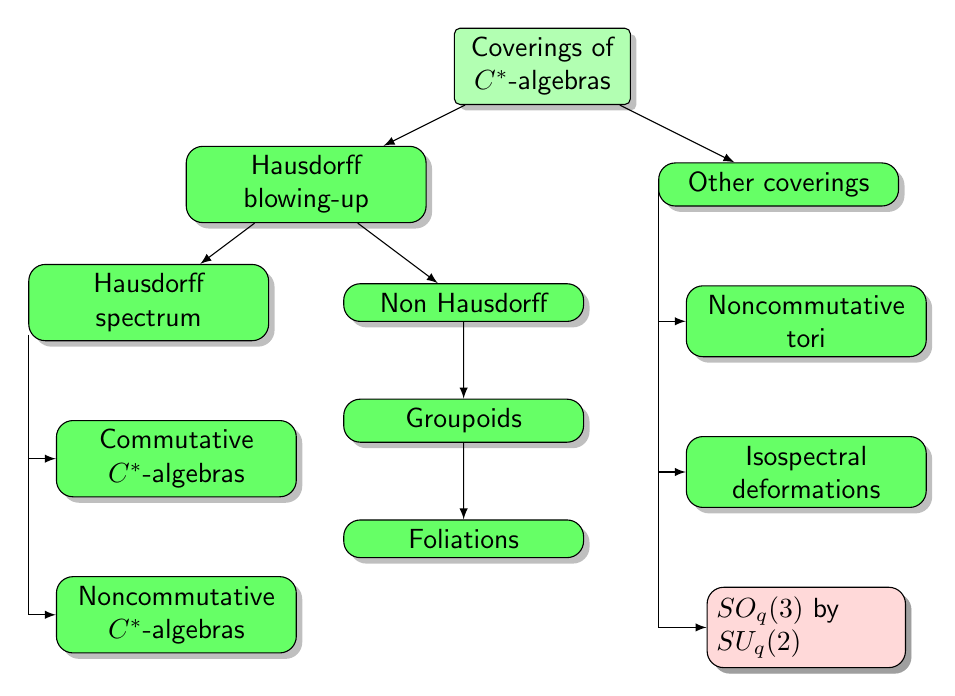
\begin{tikzpicture}[
		level 1/.style={sibling distance=60mm},
		level 2/.append style={sibling distance=40mm},
		edge from parent/.style={->,draw},
		>=latex]
		
		% root of the the initial tree, level 1
		\node[root] {Coverings of $C^*$-algebras}
		% The first level, as children of the initial tree
		child {node[level 2] (ch1) {Hausdorff blowing-up}
			child {node[level 2] (c1) {Hausdorff spectrum}}
			child {node[level 2] (c2) {Non Hausdorff}}{
				child {node[level 2] (c3) {Groupoids}}{
					child {node[level 2] (c4) {Foliations}}
				}
			}
		}
		child {node[level 2] (ch2) {Other coverings}
		};
		\begin{scope}[every node/.style={level 2}]
			\node [below = of  ch2, xshift=10pt] (ch21) {Noncommutative tori};
			\node [below = of  ch21] (ch22) {Isospectral deformations};
			\node [level 3] [below = of  ch22]  (ch23) {$SO_q(3)$ by $SU_q(2)$};
		\end{scope}	
		\begin{scope}[every node/.style={level 2}]
			\node [below = of  c1, xshift=10pt] (c11) {Commutative $C^*$-algebras};
			\node [below = of  c11] (c12) {Noncommutative $C^*$-algebras};
		\end{scope}	
		\foreach \value in {1,...,2}
		\draw[->] (c1.195) |- (c1\value.west);	
		\foreach \value in {1,...,3}
		\draw[->] (ch2.180) |- (ch2\value.west);
	\end{tikzpicture}	
	
\end{frame}
\section{Finite-fold coverings}
\begin{frame}
\huge{Finite-fold coverings} \normalsize	
	\begin{theorem} 	\alert{Alexander Pavlov, Evgenij Troitsky}
		Suppose both $\mathcal X$ and $\mathcal Y$ are compact Hausdorff connected spaces and $p :\mathcal  Y \to \mathcal X$
		is a continuous surjection. If $C(\mathcal Y )$ is a projective finitely generated Hilbert module over
		$C(\mathcal X)$ with respect to the action
		\begin{equation*}
			(f\xi)(y) = f(y)\xi(p(y)), ~ f \in  C(\mathcal Y ), ~ \xi \in  C(\mathcal X),
		\end{equation*}
		then $p$ is a finite-fold  covering.
	\end{theorem}
	It is naturally to define a finite-fold covering of $C^*$-algebras as an injective $*$-homomorphisms $A\hookto \widetilde A$ such that $ \widetilde A$-is a finitely generated Hilbert module over
	$A$. However this definition does not gives good generalizations of results  related to topological coverings.
	
\end{frame}
\begin{frame}
  \begin{definition}\label{connected_c_a_defn}
	We say that a $C^*$-algebra $A$ is \alert{connected} if it cannot be represented as a direct sum  $A \cong A' \oplus A''$ of nontrivial $C^*$-algebras $A'$ and $A''$.
	
	% (the Gelfand spectrum of the center of $M\left( A\right) $ is connected). Let $A \subset B$ be a connected subalgebra. We say that $A$ is a \alert{connected component} of $B$ if  $1_{M\left( A\right) }$ lies in the center of $1_{M\left( B\right) }$.
\end{definition}
\begin{definition}\label{connected_comp_defn}
	A connected closed two-sided ideal $A$ of  $C^*$-algebra $B$ is said to be a \alert{connected component of}  $B$ is there is a direct sum $B = A \oplus A'$ of $C^*$-algebras.
	\end{definition}
\end{frame}
\begin{frame}
   \begin{definition}\label{fin_quasi_defn}
	Let both  $A$ and  $\widetilde{A}$ are connected $C^*$-algebras, and let $\pi: A \hookto \widetilde{A}$ be an injective $*$-homomorphism of % connected	  
	$C^*$-algebras. Let $G$ be a finite  group of *-automorphisms of $\widetilde{A}$ such that 	$\pi\left(A\right) = \widetilde{A}^G\stackrel{\text{def}}{=}\left\{
	\left.a\in \widetilde{A}~\right|~ a = g a;~ \forall g \in G\right\}$.	We say that the triple $\left(A, \widetilde{A}, G \right)$ and/or the quadruple $\left(A, \widetilde{A}, G, \pi \right)$ and/or $*$-homomorphism $\pi: A \hookto \widetilde{A}$   is a \alert{noncommutative finite-fold  quasi-covering}. We write
	\be\label{fin_cov_gr_eqn}
	G\left(\left.\widetilde{A}~\right| {A} \right) \stackrel{\text{def}}{=}  	G.
	\ee
\end{definition}
\end{frame}
\begin{frame}
	\begin{definition}\label{pre_defn} \alert{Pet Ivankov}.
		Let $\pi: A \hookto \widetilde{A}$ be an injective *-homomorphism of connected  $C^*$-algebras such that following conditions hold:
		\begin{enumerate}
			\item[(a)] If $\Aut\left(\widetilde{A} \right)$ is a group of *-automorphisms of $\widetilde{A}$ then the group  
			$
			G \bydef \left\{ \left.g \in \Aut\left(\widetilde{A} \right)~\right|~ g\pi\left( a\right)  = \pi\left( a\right) ;~~\forall a \in A\right\}
			$
			is finite.
			\item[(b)] 	\be\label{cond_b_eqn}
			\pi\left( 	A\right)  = \widetilde{A}^G\stackrel{\text{def}}{=}\left\{\left.a\in \widetilde{A}~~\right|~ a = g a;~ \forall g \in G\right\}.\ee
		\end{enumerate}
		We say that the quadruple $\left(A, \widetilde{A}, G, \pi \right)$ and/or *-homomorphism $\pi: A \to \widetilde{A}$   is a \alert{noncommutative finite-fold  pre-covering}. 
	\end{definition}
	
\end{frame}
\begin{frame}
	\begin{definition}
		\alert{Petr Ivankov}
		Let $\left(A, \widetilde{A}, G, \pi \right)$ be a  noncommutative finite-fold  pre-covering. Suppose both $A$ and  $\widetilde{A}$ are unital. We say that $\left(A, \widetilde{A}, G, \pi \right)$ is an \alert{unital noncommutative finite-fold  covering} if $\widetilde{A}$ is a finitely generated projective  $A$-module.
	\end{definition}
	\begin{lemma}
		\alert{Petr Ivankov, Alexander Pavlov, Evgenij Troitsky.}
		If $\mathcal  X$ is a connected, compact, Hausdorff space then there is a natural 1-1 correspondence 
		$$
		\left(p:\widetilde{\mathcal  X}\to \mathcal  X \right)\leftrightarrow \left(C\left(\mathcal  X\right), C\left(\widetilde\sX\right), G\left(\left.\widetilde{\mathcal  X} \right|\mathcal  X\right), C_0\left(p \right)  \right).  
		$$	
		
		between finite-fold transitive coverings of $\mathcal  X$ and unital noncommutative finite-fold  coverings of $C\left(\mathcal  X\right)$.
	\end{lemma}
	A covering $p:\widetilde\sX\to \mathcal  X $ is \alert{transitive}  if for all $x \in \sX$  the group $G\left(\left.\widetilde{\mathcal  X} \right|\mathcal  X\right)$ transitively acts on $p^{-1}\left( x\right)$. 
\end{frame}

\begin{frame}
	
	Above definition and lemma can be applied to compact spaces and unital $C^*$-algebras. However there is a modification such that new definition yields noncommutative finite-fold coverings with nonunital $A$ and $\widetilde{A}$. It is proven that if $\left(A, \widetilde{A}, G, \pi \right)$ is a noncommutative finite-fold  pre-covering  then there is the natural invective $*$-homomorphism
	$$
	M\left( \pi\right): M\left( A\right)  \hookto M\left(\widetilde A \right) 
	$$
	
	\begin{definition}\label{fin_comp_defn}\alert{Petr  Ivankov}
		If $\left(A, \widetilde{A}, G, \pi \right)$ is a noncommutative finite-fold  pre-covering then it is said to be 	a \alert{noncommutative finite-fold covering with unitization} if 
		$\left(	M\left( A\right) , 	M\left( \widetilde{A}\right) , G, 	M\left( \pi\right)  \right)$ is an unital {noncommutative finite-fold covering}.
		Roughly speaking a finite-fold covering with unitization is approximated by unital one. This notion cannot be applied to coverings of a perforated plane.
		
			\end{definition}
\end{frame}
\begin{frame}
	\begin{definition}
		\alert{Petr Ivankov}.	A   noncommutative finite-fold  pre-covering $\left(A, \widetilde{A}, G, \pi \right)$ is said to be  a \alert{noncommutative finite-fold covering} if there is an increasing net $\left\{u_\lambda\right\}_{\lambda\in\Lambda}\subset M\left( A\right)_+ $  of positive elements such that
		\begin{enumerate}
			\item[(a)] There is the limit 
			$$
			\beta\text{-}\lim_{\lambda \in \Lambda} u_\lambda = 1_{M\left(A \right) }
			$$
			in the strict topology of $M\left(A \right)$,
			\item[(b)]  If for all   $\lambda\in\Lambda$ both $A_\lambda$ and  $\widetilde A_\lambda$ are $C^*$-norm completions  of $u_\lambda A u_\lambda$ and  $u_\lambda\widetilde{A}u_\lambda$ respectively then for every $\lambda\in\Lambda$ a quadruple
			$$
			\left(A_\lambda, \widetilde{A}_\lambda, G, \left.\pi\right|_{A_\lambda} :A_\lambda\to \widetilde{A}_\lambda\right)	
			$$
			is a noncommutative finite-fold covering with unitization. The action 	$G \times \widetilde{A}_\lambda\to \widetilde{A}_\lambda$, is the restriction on $\widetilde{A}_\lambda\subset \widetilde{   A}$ of the action $G\times  \widetilde{A}\to \widetilde{A}$.
		\end{enumerate}
	\end{definition}
\end{frame}
\begin{frame}
	Roughly speaking the above  Definition is an approximation of any covering by coverings with compact spaces.	
	In result one has the following theorem.
	\begin{theorem}
		\alert{Petr Ivankov}. 	Let $\mathcal X$ be a connected, locally compact, Hausdorff space.
		If the  quadruple $\left(C_0\left(\mathcal  X \right), \widetilde{A}, G,    \pi\right)$ is a noncommutative finite-fold covering then there is a connected space $\widetilde{   \mathcal X }$ and a transitive finite-fold covering  $p: \widetilde{   \mathcal X } \to \sX$ such that
		$\left(C_0\left(\mathcal  X \right), \widetilde{A}, G,    \pi\right)$ is equivalent to $\left(C_0\left( {   \mathcal X }\right), C_0\left( \widetilde{   \mathcal X }\right), G\left(\left. \widetilde{   \mathcal X } ~\right| {   \mathcal X }\right), \pi\right)$
	\end{theorem}
This Theorem has a Hausdorff blowing-up generalization.
\end{frame}

\section{Infinite coverings}
	\subsection{Basic example}
\begin{frame}
\huge{Infinite coverings} \normalsize\\
	Let $\widetilde \sX$ be a topological space with an action $  G\times \widetilde \sX\to \widetilde\sX$ of residually finite group $  G$  of properly discontinuous  group of homeomorphisms. Let $\sX \bydef \widetilde\sX/   G$ and $p: \widetilde \sX\to\sX$ be a natural covering. 	For any finite factor group $G_\la =  G/ H_\la$ we define a space $\sX_\la \bydef \widetilde \sX/ H_\la$. Then there is a category of topological spaces and finite-fold transitive coverings given by
	\be\label{top_g_x_cat_eqn}
	\mathfrak{S}_p \bydef \left\{\left\{\sX_\la\right\}_{\la \in \La}, \left\{p^\mu_\nu:\sX_\mu\to \sX_\nu\right\}_{\substack{\mu,\nu \in \La\\\mu\ge\nu}}\right\}.
	\ee
	Usage of the functor $C_0$  yields a category of $C^*$-algebras and $*$-homomorphisms given by
	\bean
	\begin{split}
		\mathfrak{S}_{C_0\left(p\right) } \bydef \\
		\left\{ \left\{ C_0\left( p_\la\right)  :C_0\left( \mathcal{X}\right)  \hookto C_0\left( \mathcal{X}_\la\right) \right\}, \left\{ C_0\left( p^\mu_\nu\right)  :C_0\left( \mathcal{X}_\mu\right)  \hookto C_0\left( \mathcal{X}_\nu\right) \right\}  \right\}.
	\end{split}
	\eean
\end{frame}
\begin{frame}
	If  $\widehat{G} \bydef \varprojlim_{\la \in \La} G\left(  \left. \sX_\la~\right|\sX \right)$ is an inverse limit of finite groups  then the group  $\widehat{G}$ is profinite. One has $\sX_\la \bydef \widetilde \sX/ \ker\left( G\left(\left. \widetilde\sX~\right|\sX \right)\to G\left(  \left. \sX_\la~\right|\sX \right)\right)$ and there is an inverse limit $\widehat \sX = \varprojlim_{\la \in \La} \sX_\la$ of topological spaces. There is a natural continuous map $\widetilde{\widehat p}: \widetilde \sX  \to \widehat \sX$. If we consider a  {final} {with respect to the family of maps} $\left\{g \circ \widehat p\right\}_{g\in \widehat{G}}$ topology on $\widehat \sX$  then we obtain a topological space $\overline \sX$.
\end{frame}
\begin{frame}

\begin{lemma}\label{top_disconnected_lem}
	Under the above hypotheses  the following conditions hold.
	\begin{enumerate}
		\item[(i)] If $\left\{g_\iota G\left(\left. \widetilde\sX~\right|\sX \right)\right\}_{\iota \in I}$   is  a set of all left  cosets of $G\left(\left. \widetilde\sX~\right|\sX \right)$ in $\widehat{G}$  then there is a natural homeomorphism 
		\be\label{top_disconnected_eqn}
		\overline \sX \cong \bigsqcup_{\iota\in I} g_\iota \widetilde\sX.
		\ee
		
		\item[(ii)] The natural map $\widetilde{\widehat p}: \widetilde \sX  \to \widehat \sX$ yields a natural inclusion $\widetilde \sX \subset \overline \sX$ such that $\widetilde \sX$ is a quasi-component  of $\overline \sX$.
		\item[(iii)] For any  a quasi-component $\widetilde \sX' \subset \overline \sX$ there is $g \in \widehat{G}$ such that $\widetilde \sX' = g \widetilde \sX$.
		\item[(iv)]  For any $\la \in \La$ the natural surjective map $\widehat p_\la: \widehat \sX \to \sX_\la$ yields a covering  $\overline p_\la: \overline \sX \to \sX_\la$ such that $\sX_\la\cong \overline\sX/ \ker \left(\widehat{G} \to G_\la \right)$. 
		\item[(v)] There is a natural bijective continuous map $\overline{\widehat p}: \overline \sX \to \widehat \sX$.
	\end{enumerate}	
\end{lemma}

\end{frame}
\begin{frame}
	\begin{definition}\label{top_disconnected_defn}
		Under the  hypotheses of the Lemma \ref{top_disconnected_lem} we say that the map $\overline p: \overline \sX  \to  \sX$  is the \alert{disconnected covering of} $p : \widetilde \sX \to \sX$. The {topological} $\overline \sX$-$\widehat  G$-{category} $\mathfrak{S}_p$ is the \alert{finite covering category of} $p : \widetilde \sX \to \sX$.
		Write
		\be\label{top_category_fin_eqn}
		\mathfrak{S}_p \bydef \left\{\left\{\sX_\la\right\}_{\la \in \La}, \left\{p^\mu_\nu:\sX_\mu\to \sX_\nu\right\}_{\substack{\mu,\nu \in \La\\\mu\ge\nu}}\right\}.
		\ee
		We say that $p : \widetilde \sX \to \sX$ is the \alert{covering inverse limit of} $\mathfrak{S}_p$
		and we write
		\be\label{top_disconnected_lim_eqn}
		\widetilde \sX \bydef \varprojlim \mathfrak{S}_p
		\ee
	\end{definition}
	\
\end{frame}

\begin{frame}
 \begin{definition}\label{g_category_defn}\alert{Petr Ivankov}
	Let $ G$ be a residually finite group. 
	Let $\left\{G_\la\right\}_{\la\in \La}$ be the indexed by a set $\La$ family of all finite factor groups of $ G$. If we define an order on $\La$ by the following way
	\bean\label{top_group_order_eqn}
	\mu \ge \nu \quad \Leftrightarrow \quad \text{there is the natural homomorphism} \quad G_\mu \to G_\nu
	\eean
	with a natural commutative diagram
	\\
	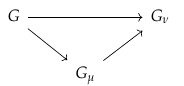
\includegraphics[scale=1]{g.png}
	\\
	then $\La$ becomes an directed set . We say that the set $\La$ is $  G$-\alert{set} and the given by $\La$ pre-ordering category  is $  G$-\alert{category}  $  G$-{category} denoted by $\La_{ G }$.
	There is the natural functor from $\La_{ G }$ to the category of finite groups and surjective homomorphisms. The element $\la_{\min }\in \La$ which corresponds to the trivial factor-group $G_{\la_{\min}}= \{e\}$ is said to be \alert{minimal}.
\end{definition}
\end{frame}
\begin{frame}
 	If  $\widehat{G}$ is a profinite group   then 
$\widehat{G} \bydef \varprojlim_{\la \in \La}  G_\la$ is an inverse limit of finite groups. The set $\La$ is directed. Indeed $\La$ is the $\widehat{G}$-set. Let $\overline A$ be a $C^*$-algebra with an action $\widehat{G}\times \overline A\to \overline A$ such that any $ g \in \widehat G$ yields an $*$-automorphism of $\overline A$.	  
Suppose that for any element $\overline a \in K\left(\overline A \right)$ of the Pedersen's ideal of $\overline A$  a series 
\be\label{infinite_covering_basic_eqn}
\sum_{	g \in \widehat{G}}g \overline a
\ee
is convergent with respect to the strict topology of $M\left(\overline A\right)$.  For any $\la \in \La$ denote by $A_\la$ a generated by elements
\be\label{basic_cov_cl_eqn}
a_\la =\bt\text{-} \sum_{	g \in \ker\left( \widehat{G}\to G_\la\right) }g \overline a
\ee
$C^*$-subalgebra of $M\left(\overline A\right)$, where  $\bt\text{-} \sum$ means a convergence  with respect to the strict topology of $M\left(\overline A\right)$. 
\end{frame}
\begin{frame}
 \begin{lemma}\label{infinite_quasi_covering_lem}
	Under the above hypotheses  all $\mu, \nu \in \La$ such that $\nu\ge\mu$ there is a natural noncommutative finite-fold quasi-covering $\left(A_\mu, A_\la, G_\nu/ G_\mu, \pi^\mu_\nu\right)$.
\end{lemma}
\end{frame}
\begin{frame}
 \begin{definition}\label{infinite_quasicovering_defn} 	Under the above hypotheses    $\la_{\mathrm{min}}\in \La$ is the minimal element and $A\bydef A_{\la_{\min}}$ then we say that the triple $\left( A, \overline A, \widehat G\right)$ is an  \alert{infinite quasi-covering}. We say that $A_\la$ is the $\la$-\alert{descent of} $\overline A$. The natural injective $*$-homomorphism $\lift_\la: A_\la \hookto M\left(\overline A \right)$ is the $\la$-\alert{lift}.
\end{definition}
\begin{definition}\label{infinite_desc_defn}
It is proven that under the above  hypotheses   for all $\la\in\La$ there is a  natural   homomorphism of $A_\la$-$A_\la$-bimodules given by
	\be\label{inf_desc_eqn}
	\begin{split}
		\desc_{\la} : K\left(\overline A \right) \to K\left(A_\la \right),\\
		\overline a \mapsto\bt\text{-} \sum_{	g \in \ker\left( \widehat{G}\to G_\la\right) }g \overline a
	\end{split}
	\ee
	where  $\bt\text{-} \sum$ means the convergence with respect to the strict topology of $M\left(\overline A\right)$. 
	We denote this homomorphism as   $\desc_{\la}$ and we say that it is  the $\la$-\alert{descent}.% If $\la_{\min}\in \La$ is the minimal element (cf. then a given by	
%	$$
%	\desc \bydef \desc_{\la_{\min}}: K\left(\overline A \right) \to K\left(A \right)
%	$$  homomorphism   of $A$-$A$-bimodules is the \alert{minimal descent}.
\end{definition}

\end{frame}

\begin{frame}
	Under the above hypotheses  there is a category $\mathfrak{S}$ such that
\begin{itemize}
	\item $\mathfrak{S}$-objects are $C^*$-algebras $A_\la$ where $\la\in \La$,
	\item $\mathfrak{S}$-morphisms are natural injective $*$-homomorphisms $\pi^\mu_\nu : A_\mu \hookto A_\nu$
	such that the diagram
	\\
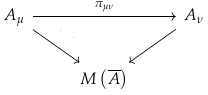
\includegraphics[scale=0.8]{ag.png}
	\\
	is commutative.
\end{itemize}

\end{frame}
\begin{frame}
 
\begin{definition}\label{algebraical_finite_covering_category_defn}
	The  above category is said to be an \alert{algebraical finite covering category} if one has:
	\begin{enumerate}
		\item [(a)] 
		any $\mathfrak{S}$-morphism $\pi^\mu_\nu : A_\mu \hookto A_\nu$ is a noncommutative finite-fold  covering,
		\item[(b)] for all $\la \in \La$ is the $\la$-{descent} $\desc_{\la} : K\left(\overline A \right) \to K\left(A_\la \right)$   is surjective, i.e. $\desc_{\la} \left(  K\left(\overline A \right)\right) = K\left(A_\la \right)$.%, moreover we require that $\desc_{\la} \left(  K\left(\overline A \right)_+\right) = K\left(A_\la \right)_+$. 
	\end{enumerate}
	We write
	\be\label{algebraical_finite_covering_category_eqn}
	\mathfrak{S}\bydef \left\{\left\{A_\la\right\}_{\la\in \La}, \left\{\pi^\mu_\nu : A_\mu \hookto A_\nu\right\}_{\substack{\mu, \nu \in \La\\\mu \le \nu}}\right\}
	\ee
	Moreover the given above infinite quasi-covering $\left( A, \overline A, \widehat G\right)$ is said to be a \alert{pre-covering of the algebraical finite covering category}  $\mathfrak{S}$.
\end{definition}


\end{frame}


\begin{frame}
	It is not clear whether pre-covering of the algebraical finite covering category is always unique. So one needs the following definition.
\begin{definition}\label{disconnected_infinite_noncommutative_covering_defn}
Roughly speaking the  \alert{disconnected infinite noncommutative covering} of $\mathfrak{S}=\left\{\left\{A_\la\right\}_{\la\in \La}, \left\{\pi^\mu_\nu : A_\mu \hookto A_\nu\right\}_{\substack{\mu, \nu \in \La\\\mu \le \nu}}\right\}$ is the union of all pre-coverings.

\end{definition}
\begin{theorem}\label{uni_dicsonnected_lem}
	For any algebraical finite covering category
$\mathfrak{S}=\left\{\left\{A_\la\right\}_{\la\in \La}, \left\{\pi^\mu_\nu : A_\mu \hookto A_\nu\right\}_{\substack{\mu, \nu \in \La\\\mu \le \nu}}\right\}$ there is the unique disconnected infinite noncommutative covering.
\end{theorem}
\end{frame}
\begin{frame}
		Let	 $\left(A, \overline{A},\widehat{G} \right)$ be a  disconnected infinite noncommutative covering of $\mathfrak{S}=\left\{\left\{A_\la\right\}_{\la\in \La}, \left\{\pi^\mu_\nu : A_\mu \hookto A_\nu\right\}_{\substack{\mu, \nu \in \La\\\mu \le \nu}}\right\}$. If $\widetilde A$ is a connected component  of $\overline{A}$, i.e. $\overline{A} = \widetilde A \oplus \widetilde A^\perp$, and
	\be\label{infinite_covering_transformation_group_eqn}
	G\left(\left.\widetilde{A}~\right| A\right)\bydef 
	\left\{\left. g \in \widehat{G}\right| \forall \widetilde a^\perp \in \widetilde A^\perp \quad g \widetilde a^\perp= \widetilde a^\perp\right\}
	\ee
	then there is a natural action
	\be\label{gta_act_eqn} 
	G\left(\left.\widetilde{A}~\right| A\right)\times \widetilde{A} \to \widetilde{A}.
	\ee
	\begin{definition}\label{good_defn}
		A  disconnected infinite noncommutative covering 	$\left(A, \overline{A},\widehat{G}\right)$ be of $\mathfrak{S}$  is \alert{good} if  following conditions hold:
		\begin{enumerate}
			\item[(a)] if both $\widetilde{A}'$ and $\widetilde{A}''$ are  {connected components} of $\overline A$ then there is  $g \in \widehat{G}$ such that $g \widetilde{A}'= \widetilde{A}''$,
			\item [(b)] if $\widetilde A$ is a   connected component of $\overline{A}$  then for any $\la \in \La$ the restriction $h_\la|_{\widetilde A}$ is an epimorphism, i. e. $h_\la\left(G\left(\left.\widetilde{A}~\right| A\right) \right) = G\left(\left. A_\la~\right|~A \right)$.
		\end{enumerate}
	\end{definition}

	\end{frame}
\begin{frame}
	\begin{definition}\label{infinite_noncommutative_covering_defn}
		If $\left(A, \overline{A},\widehat{G}\right)$ is a good  disconnected infinite noncommutative covering of $\mathfrak{S}=\left\{\left\{A_\la\right\}_{\la\in \La}, \left\{\pi^\mu_\nu : A_\mu \hookto A_\nu\right\}_{\substack{\mu, \nu \in \La\\\mu \le \nu}}\right\}$  then a connected component $\widetilde{A} \subset \overline{A}$ is said to be the \alert{inverse noncommutative limit of} $\mathfrak{S}=\left\{\left\{A_\la\right\}_{\la\in \La}, \left\{\pi^\mu_\nu : A_\mu \hookto A_\nu\right\}_{\substack{\mu, \nu \in \La\\\mu \le \nu}}\right\}$. The given by the equation \eqref{infinite_covering_transformation_group_eqn} group $G\left(\left.\widetilde{A}~\right| A\right)$  is said to be the \alert{covering transformation group}.  The triple
		\be\label{infinite_noncommutative_covering_eqn}
		\left(A, \widetilde{A}, G\left(\left.\widetilde{A}~\right| A\right)\right)
		\ee
		is said to be the  \alert{infinite noncommutative covering} or the  \alert{covering} of  $$\mathfrak{S}=\left\{\left\{A_\la\right\}_{\la\in \La}, \left\{\pi^\mu_\nu : A_\mu \hookto A_\nu\right\}_{\substack{\mu, \nu \in \La\\\mu \le \nu}}\right\}.$$ 
	\end{definition}
	
	\end{frame}
	\begin{frame}
\begin{theorem}\label{top_main_thm}
	If one has 
	\begin{itemize}
		\item the {disconnected  $\overline p: \overline \sX  \to  \sX$ covering of} a covering $p : \widetilde \sX \to \sX$ with connected $\widetilde \sX$ and a residually finite covering group $G\left(\left.\widetilde \sX~\right| \mathcal X\right)$,
		\item the finite covering category 	$\mathfrak{S}_p \bydef \left\{\left\{\sX_\la\right\}_{\la \in \La}, \left\{p^\mu_\nu:\sX_\mu\to \sX_\nu\right\}\right\}$ of $p : \widetilde \sX \to \sX$,
	\end{itemize}
	then  the given by 
	\bean\label{top_x_g_eqn}		\begin{split}
		\mathfrak{S}_{C_0\left(p\right) } \bydef \\
		\left\{ \left\{  C_0\left( \mathcal{X}_\la\right) \right\}_{\la\in\La}, \left\{ C_0\left( p^\mu_\nu\right)  :C_0\left( \mathcal{X}_\mu\right)  \hookto C_0\left( \mathcal{X}_\nu\right) \right\}  \right\}
	\end{split}
	\eean	
		
		algebraic finite covering category  is good   and the triple $$\left(C_0\left(\mathcal{X}\right), C_0\left(\widetilde \sX\right) ,G\left(\left.\widetilde \sX~\right| \mathcal X\right)\right)$$ is  the  {infinite noncommutative covering} of $\mathfrak{S}_{C_0\left( p\right) }$.
	
\end{theorem}
There is Hausdorff blowing-up generalization of this theorem.
	\end{frame}

\section{Hausdorff blowing-up and coverings}

\begin{frame}
	\huge Hausdorff blowing-up and coverings \normalsize\\
	Let $A$ be a $C^*$-algebra, and let $C_0\left(\sY \right)\subset  M\left(A \right)$ be  Hausdorff blowing-up. Let $q: \widetilde \sY\to \sY$ be a transitive covering such that $\sY = \widetilde \sY/G$ where $G$ is properly   discontinuous,  residually finite group  of homeomorphisms of $\widetilde \sY$. There is $C_0\left(\sY \right)$-valued product
\bean
\left\langle\cdot, \cdot  \right\rangle_{C_0\left(\sY \right)}: C_c \left(\widetilde \sY \right) \times C_c \left(\widetilde \sY \right)\to C_0\left(\sY \right),\\
\left(\widetilde f, \widetilde h \right) \mapsto \bt\text{-}\sum_{g\in G}\left(\widetilde f^* \widetilde h \right) 
\eean
where $\bt\text{-}\sum$ means the convergence of the series with respect to the strict topology of $M\left(C_0\left(\widetilde \sY \right)\right)$ and the natural inclusion  $C_0\left(\sY \right)\hookto M\left(C_0\left(\widetilde\sY \right)\right)$ is implied.

So $ C_c \left(\widetilde \sY\right)$ is a pre-Hilbert $C_0\left(\sY \right)$-module \end{frame}
\begin{frame}
 If $\mathscr L^2\left(C_0 \left(\widetilde \sY \right) \right)$ is a completion of $C_c \left(\widetilde \sY \right)$ with respect to the norm
 $$
 \widetilde f \mapsto \sqrt{\left\| \left\langle \widetilde f,  \widetilde f  \right\rangle_{C_0\left(\sY \right)}\right\| }
 $$
  then $\mathscr L^2\left(C_0 \left(\widetilde \sY \right) \right)$ is a $C^*$-Hilbert $C_0\left(\sY \right)$-module. If $\mathscr L^2\left(C_0 \left(\widetilde \sY \right) \right)\otimes_{C_0\left(\sY \right)} A$ is an algebraic tensor product then there is an $A$-valued product.
	\bean
	\left\langle\cdot, \cdot  \right\rangle: \left( \mathscr L^2\left(C_c \left(\widetilde \sY \right) \right)\otimes_{C_0\left(\sY \right)} A\right)\times \left( \mathscr L^2\left(C_c \left(\widetilde \sY \right) \right)\otimes_{C_0\left(\sY \right)} A\right) \to A,\\
	\left(\left(\widetilde f \otimes a \right) , \left(\widetilde h  \otimes b \right)  \right) \mapsto a^*\left\langle\widetilde f, \widetilde g \right\rangle_{C_0\left(\sY \right)} b.
	\eean
	so $\mathscr L^2\left(C_0 \left(\widetilde \sY \right) \right)\otimes_{C_0\left(\sY \right)} A$ becomes a pre-Hilbert $A$-module.
	
\end{frame}	
\begin{frame}
	 We denote by $\mathscr L^2\left(\widetilde \sY \right) _A$ the $C^*$-Hilbert $A$-module which is a completion  of  $\mathscr L^2\left(C_0 \left(\widetilde \sY \right) \right)\otimes_{C_0\left(\sY \right)} A$ with respect to the norm given by
 $$
\widetilde f \otimes a \mapsto \sqrt{\left\| \left\langle \widetilde f \otimes a,  \widetilde f \otimes a  \right\rangle\right\| }
$$	
 There are both a left  action 	$C_0 \left(\widetilde \sY \right)\times \mathscr L^2\left(\widetilde \sY \right) _A\to \mathscr L^2\left(\widetilde \sY \right) _A$ and the right action $\mathscr L^2\left(\widetilde \sY \right) _A\times A \to \mathscr L^2\left(\widetilde \sY \right) _A$ such that $\mathscr L^2\left(\sY\right)_A$ is $C_0 \left(\widetilde \sY \right)$-$A$-bimodule. These actions induce injective homomorphisms of $C^*$-algebras
	\bean
	\varphi_A : A \hookto \End^*_A\left( \mathscr L^2\left(\widetilde \sY \right)_A\right), \\
	\label{blowing_c_h_eqn}
	\varphi_{\widetilde \sY} : C_0 \left(\widetilde \sY \right) \hookto \End^*_A\left( \mathscr L^2\left(\widetilde \sY \right)_A\right)
	\eean
	where $\End^*_A\left( \mathscr L^2\left(\widetilde \sY \right)_A\right)$ is the $C^*$-algebra of adjointable  endomorphisms
	\end{frame}
	\begin{frame}
	There is a homomorphism 
	\be\label{blowing_tensor_eqn} 
	\begin{split}
		\varphi^{\widetilde \sY}_A: C_0\left( \widetilde \sY \right)\otimes_{C_0\left(\sY\right) } K\left( A\right) \to \End^*_A\left( \mathscr L^2\left(\widetilde \sY \right)_A\right),\\
		\sum_{j=1}^n 	\widetilde f_j \otimes a_j \mapsto 	\sum_{j=1}^n 	\varphi_{\widetilde \sY}\left( \widetilde f_j\right) \varphi_A\left(a_j \right)
	\end{split}
	\ee
	of  $C_0\left( \widetilde\sY\right)$-$A$-bimodules. Since both $C_c\left(\widetilde \sY \right)$ and   $K\left(A \right)$ are dense in $C_0\left(\widetilde \sY \right)$ and  $A$ respectively the $*$-homomorphism \eqref{blowing_tensor_eqn} can be uniquely extended up to a  $C_0\left( \widetilde\sX\right)$-$A$-bimodule homomorphism 
	\be\label{blowing_tensoar_eqn} 
	\begin{split}
		\psi^{\widetilde \sY}_A: C_0\left( \widetilde \sY \right)\otimes_{C_0\left(\sY\right) } A \to \End^*_A\left( \mathscr L^2\left(\widetilde \sY \right)_A\right)
	\end{split}
	\ee
	such that the $C^*$ closure of $\varphi\left(  C_c\left( \widetilde \sY \right)\otimes_{C_0\left(\sY\right) } K\left( A\right)\right)$ coincides with\\  	$\varphi'\left(  C_c\left( \widetilde \sY \right)\otimes_{C_0\left(\sY\right) } A\right) $ one.
\end{frame}
\begin{frame}
\begin{definition}\alert{Petr Ivankov}
	If 	$C_0\left( \widetilde\sY\right)$-$A$-bimodule
	\be\label{blowing_prods_eqn}
	\varphi^{\widetilde \sY}_A\left(C_c\left( \widetilde \sY \right)\otimes_{C_0\left(\sY\right) } K\left( A\right) \right)\subset  \End^*_A\left( \mathscr L^2\left(\widetilde \sY \right)_A\right)
	\ee	
	 is a $*$-subalgebra of $\End^*_A\left( \mathscr L^2\left(\widetilde \sY \right)_A\right)$
	then  we say that the covering $q: \widetilde{\sY}\to \sY$ is $A$-\alert{regular}.  
	\end{definition}
	The above definition is very interesting because
	\begin{itemize}
		\item it is related to coverings of $C^*$-algebras,
		\item it is an algebraic formulation of the geometric notion of coverings of groupoids.
	\end{itemize}
	
\end{frame}
	\subsection{Finite-fold coverings}
	
	\begin{frame}
If  a covering $q: \widetilde{\sY}\to \sY$ is $A$-{regular} then we denote by $A_0\left( \widetilde \sY\right)$ the $C^*$-norm completion of $\varphi^{\widetilde \sY}_A\left(C_c\left( \widetilde \sY \right)\otimes_{C_0\left(\sY\right) } K\left( A\right) \right)$. There is an injective $*$-homeomorphism
$
A_b\left(q \right) : A \hookto M\left(A_0\left( \widetilde \sY\right) \right) 
$. In particular if the covering $q$ is finite-fold then there is an injective $*$-homomorphism $
A_0\left(q \right) : A \hookto A_0\left( \widetilde \sY\right).
$
\begin{theorem}\label{blowing_sufficient_covering_thm}
	Let $C_0\left(\sY \right) \hookto M\left(A \right)$ be a Hausdorff blowing-up  with  locally connected $\sY$, and let 
	$q: \widetilde\sY \to \sY$  be a finite-fold transitive $A$-regular covering  with connected $\widetilde \sY$. If	$A_0\left(q\right) : A \hookto	 A_0\left( \widetilde \sY\right)$ is a {finite}-$q$-{lift} (cf. Definition   then the quadruple $$\left(A,	 A_0\left( \widetilde \sY\right), G\left(\left.\widetilde \sY\right|\sY \right), A_0\left(q\right)\right)$$ is a noncommutative finite-fold covering.
\end{theorem}
This theorem is a generalization of the theorem related to noncommutative finite-fold coverings of commutative $C^*$-algebras.

\end{frame}

\subsection{Infinite coverings}
\begin{frame}
\begin{theorem}\label{blowing_sufficient_covering_inf_thm} % {blowing_inf_cov_thm}
	Let $C_0\left( \sY\right) \hookto M\left( A\right) $ be    Hausdorff blowing-up, and
	let $q:\widetilde \sY \to \sY$ be an $A$-regular transitive covering with connected $\widetilde \sY$ and residually finite group  $G\left(\left.\widetilde \sY\right|\sY \right)$ of covering transformations, then one has
	\begin{enumerate}

		\item[(i)] there is a  {finite covering category of} $q : \widetilde \sY \to \sY$  given by
		\bean\label{blowing_category_fin_eqn}
		\mathfrak{S}_p \bydef \left\{\left\{\sY_\la\right\}_{\la \in \La}, \left\{q^\mu_\nu:\sY_\mu\to \sY_\nu\right\}_{\substack{\mu,\nu \in \La\\\mu\ge\nu}}\right\}
		\eean
		yields an algebraical finite covering category 
		\bean\label{blowing_algebraical_finite_covering_category_eqn}
		\mathfrak{S}_{A_0\left(q \right) }\bydef \left\{\left\{A_0\left( \sY_\la\right) \right\}_{\la\in \La}, \left\{A_0\left( q^\nu_\mu\right)  : A_0\left( \sY_\mu\right) \hookto A_0\left( \sY_\nu\right)\right\}_{\substack{\mu, \nu \in \La\\\mu \le \nu}}\right\}
		\eean
 such that 	a triple $\left(A, A_0\left(\overline\sY \right), \widehat{G} \right)$  is a {pre}-{covering of algebraical finite covering category}  $\mathfrak{S}_{A_0\left(q \right) }$ (cf. Definition \ref{algebraical_finite_covering_category_defn}), 
		\item[(ii)] if the triple $\left(A, A_0\left(\overline\sY \right), \widehat{G} \right)$   is the  \alert{infinite noncommutative pre-covering} of  $\mathfrak{S}_{A_0\left(q \right) }$.
	\end{enumerate}
\end{theorem}
\end{frame}
\begin{frame}
	\huge Problems \normalsize
	\begin{enumerate}
		\item The above theorem is a generalization of the theorem related to infinite coverings of commutative $C^*$-algebras. 
		\item The above theorem does not give infinite noncommutative coverings, it yields pre-coverings only.
		\item In some specializations it is proven that  pre-coverings are coverings.
		\item Maybe be all  pre-coverings are indeed coverings but now it is not known.
	\end{enumerate}
\end{frame}


\section{Algebras of groupoids}

\begin{frame}
	\begin{definition}
	% 104
	A \alert{groupoid} consists of a set $\G$, a distinguished subset $\G^0\subset\G$, two maps
	$r, s : \G\to \G^0$ and a law of composition
	$$
	\circ: \G^2\bydef\left\{\left.\left(\ga_1,\ga_2 \right) \in \G\times\G~\right| s\left(\ga_1\right)= r\left(\ga_2\right)\right\}\to \G
	$$
	such that
	\begin{enumerate}
		\item $s\left(\ga_1\circ\ga_2\right)=s\left(\ga_2\right), \quad r\left(\ga_1\circ\ga_2\right)=r\left(\ga_1\right)\quad \forall\left(\ga_1, \ga_2 \right) \in \G$
		\item $s\left(x\right)=r\left(x\right)=x \quad\forall x\in\G^0$
		\item $\ga\circ s\left(\ga\right)= r\left(\ga\right)\circ\ga = \ga\quad \forall\ga\in\G$
		\item $\left( \ga_1\circ\ga_2\right) \circ\ga_3=\ga_1\circ\left( \ga_2\circ\ga_3\right) $
		\item Each $\ga \in\G$ has a two-sided inverse $\ga^{-1}$, with $\ga\circ\ga^{-1}=r\left(\ga\right)$, $\ga^{-1}\circ\ga=r\left(\ga\right)$.
	\end{enumerate}
	The maps $r$, $s$ are called the \alert{range} and \alert{source} maps.
\end{definition}

\end{frame}
\begin{frame}
		\begin{definition}\label{groupoid_topological_defn}
		A \alert{topological groupoid} consists of a groupoid $\G$ and a topology compatible with the groupoid structure:
		\begin{enumerate}
			\item [(a)] $\G \to \G \quad x \mapsto x^{-1}$ is continuous,
			\item [(b)] $\G^2\to \G\quad \left(x,y\right)\mapsto xy$ is continuous where $\G^2$ has the induced topology from $\G \times \G$.
		\end{enumerate}
	\end{definition}
\begin{definition}
	For $u, v\in \G^0$, $~\G^u\bydef r^{-1}\left( u\right)$,  $~\G_v\bydef s^{-1}\left( v\right)$  $~\G^u_v\bydef \G^u\cap \G_v$ and
	$\G(u) = G^u_u$ which is a group, is called  the \alert{isotropy  group} at $u$.
\end{definition}
	
\begin{definition}\label{groupoid_covering_defn}
	Let $p : \widetilde{\G}\to \G$ be a morphism of groupoids. An ordered pair
	$\left( \widetilde{\G}, p\right)$ is a \text{covering groupoid} if for each object $\widetilde u \in \widetilde{\G}$ the restriction of $p$
	$$
	\widetilde{\G}^{\widetilde{u}}\to {\G}^u
	$$
	is bijection. The morphism $p$ is called the \alert{covering}. 
\end{definition}
\end{frame}

\begin{frame}

The existence of covering is relevant to the lifting problem
	\newline
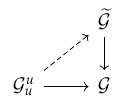
\includegraphics[scale=0.7]{lifting.png}
\newline
	One can find obstructions of it in the fundamental group $\pi_1\left( \G^u_u, u \right)$
	\begin{definition}
	If $\G$ is a groupoid then a covering $\widetilde \sY \to \G^0$ is $\G$-\alert{regular} if there is a covering of groupoids $\widetilde{\G}\to \G$ such that the natural map $\widetilde \G^0 \to \G^0$ is equivalent to $\widetilde \sY \to \G^0$ one.
	\end{definition}
\end{frame}	
\section{Algebra and geometry}
\begin{frame}
	One has
	\begin{enumerate}
		\item 	For any groupoid $\G$ any 2-cycle on $\G$ any faithful representation $C_c\left( \G, \sigma\right)\to B\left( \H\right)$   there is a $C^*$-algebra
		$C^*_r\left( \G, \sigma\right)$ with Hausdorff blowing-up $C_0\left(\G^0 \right) \subset M\left(C^*_r\left( \G, \sigma\right) \right)$ 
		\item 	Any $\G$-regular covering $\widetilde \sY \to \G^0$ is $C^*_r\left( \G, \sigma\right)$-regular. So any geometric covering of groupoid $\widetilde{\G}\to \G$ corresponds to a noncommutative covering of its $C^*$-algebra $C^*_r\left( \G, \sigma\right)$.
		\item Coverings of topological spaces and groupoids are specializations of the single theory.
	\end{enumerate}
	
	

\end{frame}


\begin{frame}
	Given a $\G$-module bundle $( A , L )$, one can form the following cochain complex. Let
	us first define $\G^n$ for any $n\in\N$. The sets $\H^0$ , $\G^1\bydef \G$ and $\G^2$ have already been defined. For $n> 2$, $\quad \G^n$ is the set of $n$-tuples $(x_0 . . . . . x_{n-1}) \in \G\times...\times \G$ such that for $
	j = 1 , . . . , n - 1$ , $\quad x_j$ is composable with its left  neighbor. A $n$-cochain is a function from $G^n$ to $A$ which satisfies the conditions
	\begin{enumerate}
		\item[(i)] $p\circ f(x_0 . . . . . x_{n-1}) = d(x_0)$ and
		\item[(ii)] if $n > 0$ and for some $j = 0, . . . , n - 1$ , $\quad x_0 \in \G^0$, then $f ( x_0, ..., x_j , ..., x_{n-1})\in A^0$.
	\end{enumerate}
	\end{frame}
	\begin{frame}
	The set $C^n\left(\G, A\right)$ of $n$-cochains is an Abelian group under point-wise addition. The
	sequence 
	\bean
	0 \to C^0\left( \G, A\right)\to C^0\left( \G, A\right)\to C^1\left( \G, A\right)\to...\to  C^n\left( \G, A\right) \xrightarrow{\delta^n} C^{n + 1}\left( \G, A\right)\to ...
	\eean
	where 
	\bean
	\begin{split}
		\delta^0f(x)\bydef L(x)\quad  f\circ s(x) - f \circ r ( x ),\\
		\delta^n(f(x_0 ,..., x_n) = L ( x_0 ) f ( x_1,..., x_n) +\\+ \sum_{j=1}^n (-1)^j
		f ( x_0 ,..., x_{j-1}x_j . . . . . x_{n-1})+(-1)^{n-1} f ( x_0 , . . . , x_{n-1}) \quad  n > 0,
	\end{split}
	\eean
	
	is a cochain complex.
	
\begin{definition}\label{groupoid_cocycle_defn}
	The group of $n$-cocycles of this complex will be denoted by $Z^n(\G,A)$,
	the group of $n$-coboundaries will be denoted by $B^n(\G,A)$ and the $n$-th cohomology group
	$Z^n(\G,A)/B^n(\G,A)$ will be denoted by $H^n(\G,A)$.
\end{definition}
\end{frame}
\begin{frame}

\begin{definition}
Let $\G$ be a locally compact  groupoid. A \alert{left  Haar system} for $\G$
consists of measures $\left\{\left.\la^u \right| u \in \G^0\right\}$ on $\G$ such that
\begin{enumerate}
	\item [(a)] the support $\supp\la^u$ of the measure $\la^u$ is $\G^u$,
	\item [(b)]  (continuity) for any $f \in C_c\left(\G\right)$, $u \mapsto \la(f)(u) = \int f d\la^u$ is continuous, and
	\item [(c)]  (left invariance) for any $x\in \G$ and any $f \in  C_c(\G )$, $\int  f ( x y ) d\la^{s(x)}(y) =
	\int f(y)d\la^{r(x)}(y)$.
	
\end{enumerate}
\end{definition}
\end{frame}
\begin{frame}
		If the groupoid $\G$ is Hausdorff then the space $C_c\left( \G\right)$ of functions with compact support is well known. If not and $\G$ corresponds to a foliation then  there are two  different generalizations of  the space of functions  $C_c\left( \G\right)$  with compact support. Both definitions yield isomorphic $C^*$-algebras.
	Let $\G$ be a locally compact groupoid with left  Haar system $\left\{\la^u\right\}$ and let $\sigma$ be a continuous 2-cocycle in $Z^2\left(\G, \T\right)$. Suppose that the space $C_c\left( \G\right)$ is defined.
If for $f ,g \in C_c(\G)$, we define
\bean
\begin{split}
	f * g \left(x\right)\bydef 
	\int f ( x y ) g \left( y^{-1}\right)\sigma\left(xy, y^{-1} \right) d\la^{d(x)}(y),\\
	f^* ( x ) \bydef \overline{f ( x^{ -1})}~\overline{\sigma\left(x, x^{-1} \right)}, 	
\end{split}
\eean
then we obtain a $*$-algebra denoted by $C_c(\G, \sigma)$.


\end{frame}
\section{Coverings of groupoids}
\begin{frame}
	\begin{definition}\label{groupoid_lift_defn}
		Let $\G$ be a groupoid such that the space $\G^0$ is Hausdorff.
		Let $q: \widetilde \G^0 \to \G^0$ be transitive covering
		and let $\widetilde \G^0\times_{\G^0}\G$ be pullback where the map $s : \G \to \G^0$ is implied. We say that the covering  $q$ is $\G$-\alert{regular} if there is  the groupoid $\widetilde \G^0$ with homeomorphism $\widetilde \G\cong \widetilde \G^0\times_{\G^0}\G$ such that the natural continuous map 
		\be\label{groupoid_lift_eqn}
		q_\G: \widetilde \G \to \G
		\ee
		is a covering. The groupoid $\widetilde \G$ is the $q$-\alert{lift} of $\G$. 	A $p$-\alert{topology} on $\widetilde\G$ is such that both maps $q_\G$ and $s:  \widetilde\G \to \widetilde\G^0$ are continuous.
	\end{definition}
\end{frame}
\begin{frame}

	Let $\G$ be a locally compact groupoid, and let   $p: \widetilde \G^0 \to \G^0$ is a $\G$-{regular} covering. If  $\widetilde\G$ is  the $p$-{lift} of $\G$  then $\widetilde\G$ is locally compact. Let $\left\{\la^u \left| u \in \G^0\right.\right\}$ be a left  Haar system for $\G$. For any $\widetilde u \in \widetilde\G^0$ there is a homeomorphism $\widetilde \G^{\widetilde u} \cong \G^{p\left(\widetilde u \right) }$. Using it  for any $\widetilde u$ one can  naturally construct a measure $\widetilde  \la^{\widetilde u}$ on $\widetilde \G$. It follows that
	\begin{enumerate}
		\item [(a)] the support $\supp \widetilde  \la^{\widetilde u}$ of the measure $\widetilde  \la^{\widetilde u}$ is $\widetilde \G^{\widetilde u}$,
		\item [(b)]  (continuity) for any $\widetilde f \in C_c\left(\widetilde \G\right)$, $\widetilde u \mapsto \widetilde\la(\widetilde f)\left( \widetilde u\right)  = \int \widetilde f \widetilde d\la^{\widetilde u}$ is continuous, and
		\item [(c)]  (left invariance) for any $\widetilde x\in \widetilde \G$ and any $\widetilde f \in  C_c(\widetilde \G )$, $\int \widetilde  f \left(  \widetilde x \widetilde y \right)  d\la^{s(\widetilde x)}\left( \widetilde y\right)  =
		\int \widetilde f\left( \widetilde y\right) d\la^{d\left( \widetilde x\right) }\left( \widetilde y\right) $.
	\end{enumerate}
	From these circumstances it turns out that $\left\{\widetilde  \la^{\widetilde u}\left| \widetilde u \in \widetilde \G^0\right.\right\}$ is a left  Haar system for $\widetilde{\G}$.

\begin{definition}\label{groupoid_haar_lift_defn}
	Under above hypotheses we say that the left  Haar system $\left\{\widetilde  \la^{\widetilde u}\left| \widetilde u \in \widetilde \G^0\right.\right\}$ is the $p$-\alert{lift} of $\left\{\la^u \left| u \in \G^0\right.\right\}$.
	\end{definition}
\end{frame}
\begin{frame}
If $\sigma$ is a continuous 2-cocycle in $Z^2\left(\G, \T\right)$ then there is a map
	\bean
	\begin{split}
		\widetilde \sigma: \widetilde \G^2 \to \T,\\
		\left(\widetilde x_0, \widetilde x_1 \right) \mapsto \left(q_\G\left( \widetilde x_0\right), q_\G\left( \widetilde x_1\right)\right). 
	\end{split}
	\eean
It follows that 
	$$
	\forall \left(\widetilde x_0, \widetilde x_1 \right) \in \widetilde \G^2\quad \dl^2 \widetilde \sigma \left(\widetilde x_0, \widetilde x_1 \right)=\dl^2  \sigma \left(q_\G\left( \widetilde x_0\right), q_\G\left( \widetilde x_1\right)\right)= 1,
	$$
	i.e. $\widetilde \sigma$ is  a continuous 2-cocycle
\begin{definition}\label{groupoid_cocycle_lift_defn}
	We say that the continuous 2-cocycle $\widetilde \sigma\in Z^2\left(\G, \T\right)$ is the $q$-lift of $\sigma$.
\end{definition}
	If a groupoid $\G$ is locally compact then any $q$-lift of $\G$ is locally compact with respect to $p$-topology.
\end{frame}
\begin{frame}
	\begin{definition}
		
		Let $\sX$ be a locally compact Hausdorff space, and let $C_c\left(\sX\right)$ denote the	space of continuous, compactly supported functions on $\sX$. The natural	topology on $C_c\left(\sX\right)$ is the \alert{inductive limit topology}, defined as follows. A net	$\left\{f_\a\right\}$ in $C_c\left(\sX\right)$ converges to $f$ if there is a compact set $K\subset\sX$ containing	the supports of all $f_\a$ and $f$, and such that $f_\a$ converges uniformly to $f$ on$K$.
	\end{definition}
	
	\begin{definition}\label{groupoid_representation_defn}
		%1.3. D e f i n i t i o n : 
		A \alert{representation} of $C_c\left(\G, \sigma\right)$ on a Hilbert space $\H$ is a $*$-homomorphism $L : C_c\left(\G, \sigma\right) \to B\left(\H \right)$ which is continuous when $C_c\left(\G, \sigma\right)$ has the inductive limit 
		topology  and $B\left(\H \right)$  the weak operator topology  and is such that the linear  span of
		$$
		L\left(f \right) \xi , \quad f \in C_c\left(\G, \sigma\right), \quad \xi \in \H
		$$
		is dense in $\H$.
	\end{definition}
	
	
\end{frame}
\begin{frame}
	\begin{lemma}\label{groupoid_mult_repr_lem}
		%1.13. Lemma : 
		If $L$ is a representation of $C_c\left(\G, \sigma\right)$, there exists a unique representation
		$M$ of $C_c\left(\G^0\right)$ such that for every $h \in C_c\left(\G^0\right)$ and every $f\in C_c\left(\G, \sigma\right)$, $L\left(h f \right)= M\left(h \right)L\left(f \right)$  and
		$L\left(fh \right)= L\left(f \right)M\left(h \right)$. 
	\end{lemma}
	
	If $\G$ is locally compact groupoid with a continuous 2-cocycle in $Z^2\left(\G, \T\right)$ and a left  Haar system $\left\{\la^u\left| u \in \G^0\right.\right\}$  (cf. Definition then there is a $*$-algebra $C_c\left(\G, \sigma \right)$
	If  $\rho: 	C_c\left(\G , \sigma \right)\to B\left(\H \right)$ is a representation then there is a $C^*$-seminorm 
	\bean
	\begin{split}
		\left\|\cdot  \right\|_\rho :   	C_c\left(\G , \sigma \right)\to \mathbb{R},\\
		a \mapsto \left\|\rho\left( a \right)  \right\|
	\end{split}
	\eean
	We suppose that $\rho$ is \alert{faithful}, i.e. $a \neq 0\quad \Rightarrow \quad \rho_c\left(a \right) \neq 0$. The completion of  $C_c\left(\G , \sigma \right)$ with respect to 	$\left\|\cdot  \right\|_\rho$ is a $C^*$-algebra denoted by $C^*_\rho\left(\G , \sigma \right)$. From the Lemma it follows that there is \alert{Hausdorff blowing-up} $C_0\left(\G^0 \right) \subset C^*_\rho\left(\G , \sigma \right)$.
\end{frame}
\
\end{document}























